% Compact PGFPlots panel for sampled surface11 BSC GEXIT derivative.
% Requires \usepackage{pgfplots} and \pgfplotsset{compat=1.18}.
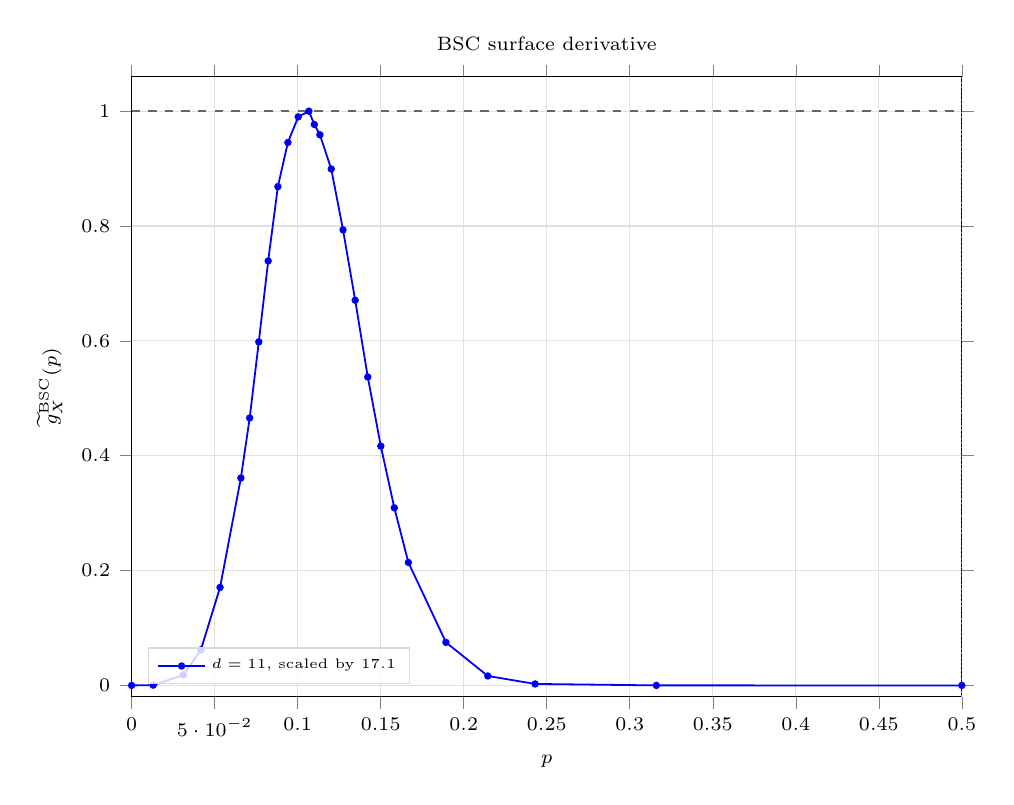
\begin{tikzpicture}
\begin{axis}[
  name=scaledBSCGEXITSurface11Axis,
  width=\linewidth,
  height=0.78\linewidth,
  title={BSC surface derivative},
  title style={font=\scriptsize},
  xlabel={$p$},
  ylabel={$\widetilde g_X^{\rm BSC}(p)$},
  xmin=0, xmax=0.5,
  ymin=-0.02, ymax=1.06,
  grid=both,
  major grid style={black!12},
  minor grid style={black!6},
  tick align=outside,
  tick label style={font=\scriptsize},
  label style={font=\scriptsize},
  legend cell align={left},
  legend style={draw=black!15, fill=white, fill opacity=0.82, text opacity=1, at={(0.02,0.02)}, anchor=south west, font=\tiny},
]
\addplot[black!60, densely dotted, line width=0.55pt, forget plot] coordinates {(0.5,-0.02) (0.5,1.06)};
\addplot[black!60, dashed, line width=0.55pt, forget plot] coordinates {(0,1) (0.5,1)};
\addplot+[color=blue, mark=*, mark size=1.0pt, line width=0.65pt]
coordinates {(0,0) (0.0129868620555,0.000489295127719) (0.0311244603048,0.0182801214824) (0.0416926902737,0.0619626504983) (0.0532390407768,0.170616523071) (0.0657867063546,0.361206087629) (0.0710958755299,0.465749190601) (0.0765765344037,0.598275401311) (0.0822333323659,0.739189969968) (0.0880715694979,0.868645530951) (0.0940972433461,0.945423650848) (0.100317108961,0.990101475235) (0.106738753821,1) (0.110027864438,0.976861579032) (0.113370689941,0.958927491273) (0.120222466333,0.899311860544) (0.127304805976,0.793345212762) (0.134629772869,0.670760529783) (0.142210976498,0.537171758217) (0.150063823499,0.416778648671) (0.158205829694,0.309263528139) (0.166657010397,0.214165175666) (0.189297705371,0.0749600137015) (0.21450174486,0.0164472625098) (0.243003853809,0.00256666763295) (0.316019346324,5.45603810413e-05) (0.5,0)};
\addlegendentry{$d=11$, scaled by $17.1$}
\end{axis}
\end{tikzpicture}
